\documentclass[12pt]{article}
\usepackage{times}
\usepackage{color}
\usepackage{graphicx}
\usepackage{authblk}
\usepackage{amsmath}
%\usepackage[maxbibnames=99]{biblatex}
%\usepackage{setspace}
%\usepackage{geometry}
\usepackage[font={sf,small}]{caption}
%\usepackage{setspace}
%\usepackage{geometry}
%\usepackage{hyperref}
%\hypersetup{
%    colorlinks,
%    citecolor=black,
%    filecolor=black,
%    linkcolor=black,
%    urlcolor=black
%}
%\geometry{letterpaper}
\usepackage[authoryear, round,sort,comma,numbers]{natbib}
\usepackage{apalike}
\usepackage{tabularx}

\usepackage{amssymb}
%\usepackage{epstopdf}
\usepackage{float}
%\DeclareGraphicsRule{.tif}{png}{.png}{`convert #1 `dirname #1`/`basename #1 .tif`.png}

\newcommand{\specialcell}[2][c]{%
	\begin{tabular}[#1]{@{}c@{}}#2\end{tabular}}
\setlength{\textheight}{9.3in}
\setlength{\textwidth}{7in}
\setlength{\footskip}{0.5in}
\setlength{\topmargin}{-0.5in}
\setlength{\headheight}{0.2in}
\setlength{\headsep}{0in}
\setlength{\parindent}{1pc}
\setlength{\oddsidemargin}{-0.25in}
\setlength{\evensidemargin}{-0.25in}
\renewcommand{\baselinestretch}{1.5}


\title{A behavioral investigation of how rodents solve the explore-exploit tradeoff}

\author[1]{Siyu Wang}
\author[2]{Blake Gerken}
\author[2]{Julia R. Wieland}
\author[1,3]{Robert C. Wilson}
\author[1,4,5]{Jean-Marc Fellous}

\affil[1]{Department of Psychology, University of Arizona}
\affil[2]{Neuroscience and Cognitive Science Program, University of Arizona}
\affil[3]{Cognitive Science Program, University of Arizona}
\affil[4]{Program in Applied Mathematics, University of Arizona}
\affil[5]{Neuroscience Graduate Interdisciplinary Program, University of Arizona}
\date{}

\providecommand{\keywords}[1]
{
  \small
  \textbf{\textit{Keywords---}} #1
}

\begin{document}
\maketitle
\newpage
%	\subsectionmark{1}
%	\begin{abstract}
%		
%	\end{abstract}

%\keywords{explore-exploit decision,  directed exploration, random exploration}
	\normalsize
\newpage
\section*{Introduction}
Humans and animals constantly face the dilemma of choosing between exploiting options that are known to be good and exploring unknown options in the hope of discovering better options for the future. Humans face it when making decisions from simple choices like deciding whether to explore a new restaurant for dinner, to important life decisions like deciding whether to explore a new career, while animals face it when deciding whether to explore and forage for food, territory or mate. The cognitive ability to balance exploration and exploitation is vital to animal and human's survival and success. In recent years, the study of explore-exploit decisions in humans and animals have become an active field \citep{Mehlhorn2015, Wilson2020}. 

Although optimal solution to explore-exploit decisions is in general computationally intractable  \cite{Bellman1954}, humans and animals are thought to use approximations or heuristics in making explore-exploit decisions. Previous research suggested both an information-driven strategy known as 
directed exploration in which action is biased towards the more uncertain option \citep{Meyer1995, Banks1997, Frank2009, Steyvers2009, Lee2011,Payzan-Lenestour2012,Zhang2013, Wilson2014, Krebs1978}, and an error-driven strategy known as random exploration in which exploratory actions with suboptimal estimates of value will be chosen by chance \citep{songbird1, songbird2, Wilson2014, Gershman2018, Gershman2019}. In particular, \cite{Wilson2014} showed that humans are able to adapt the extent to which they explore with the horizon context, i.e. the number of future choices remaining. Horizon adaptation is thought to be a hallmark of exploration. 

Relatively few studies have investigated how animals, in particular rodents, make explore-exploit decisions. To study such behavior, almost existing rodent explore-exploit studies used a reversal learning paradigm. In the reversal learning design, animals choose between two options where one is better than the other, this can be options with high vs low costs \citep{Beeler2010}, options with high reward magnitudes associated with low delay time vs low reward associated with high delay \citep{Laskowski2016}, binary reward options with high vs low probabilities  \citep{Parker2016, Cinotti2019, Verharen2020}. As animals explore the two options they will eventually converge to the better option and keep exploiting that option, until the outcome of the two options are reversed. Deviating from the previously exploit option after reversal is considered exploration in these tasks. Rodents are reported to use a win-stay lose-shift strategy which is effective in solving these reversal learning problems. Most of these tasks are implemented in a chamber box. 

% In the monkey literature, drifting bandits are used to study explore-exploit decisions. 

However, these reversal learning designs have several limitations. Firstly, the scope of "exploration" being studied is limited, as win-stay lose-shift is a very model-free exploration strategy which works well for reversal learning, planning and model-based exploration can not be observed in such designs. Secondly, going away from a current bad option is confounded with exploring a novel option for information. Thirdly, there is a gap between the human and rodent literature, few papers have used comparable tasks in humans and rodents. It is important to understand whether the same exploration strategy is used between humans and rodents to understand how translatable rodent neural results are to humans.   % model-based measures of exploration as opposed to having a clean model-free measure.


%Exploration in rodents is sometimes also studied in the sense of spatial exploration with no explicit reward function or goal function \citep{Braz2015}. 

% preprint action sequence \citep{Koralek2019}

In the current study, we partially addressed these limitations by designing a novel open-field task in which rodents choose between two locations that offer fixed different amount of sugar water. They are guided to one location first, and the extent to which they explore the unvisited location in their initial choice serves as a measure of exploration. In particular, rats performed the task in both a short and a long horizon condition. Using an open-field, we are able to use two sets of different locations alternatively as new games start as opposed to having to reverse the reward conditions at the same set of locations. Using rewards of different magnitudes instead of probability, we are taking the uncertainty in the value estimate of actions out of the equation, and as a result, exploration can be defined in a clean way that dose not depend on modeling. By looking at the extent to which rats go to the unvisited location at their initial choices, we are able to directly quantify information-driven exploration. We also ran a human version of an identical task except that humans are choosing between two slot machines that give out different amount of reward points, so we are able to compare rodent behavior directly with humans in this task. Particular, we assessed whether rats use model-based planning in exploration by evaluating whether they explore differently in a short vs long horizon context. 

\section*{Methods}
\subsection*{Animals} 
4 Brown Norwegian rats were used in the experiment. All rats were male between 6 and 7 months of age at the start of the experiment. All rats were obtained from vendor XXX. All rats were housed under reverse 12:12 light cycles. All animal procedures were approved by XXX at University of Arizona.
 
\subsection*{Human participants}
XXX participants (age XXX) participated in the experiment. All participants are from the undergraduate psychology subject pool who earn credits for participation in this study. The human experiment is approved by the University of Arizona  Institutional Review Board.

\subsection*{Behavioral Task}  
\begin{figure}[H]
	\begin{center}
			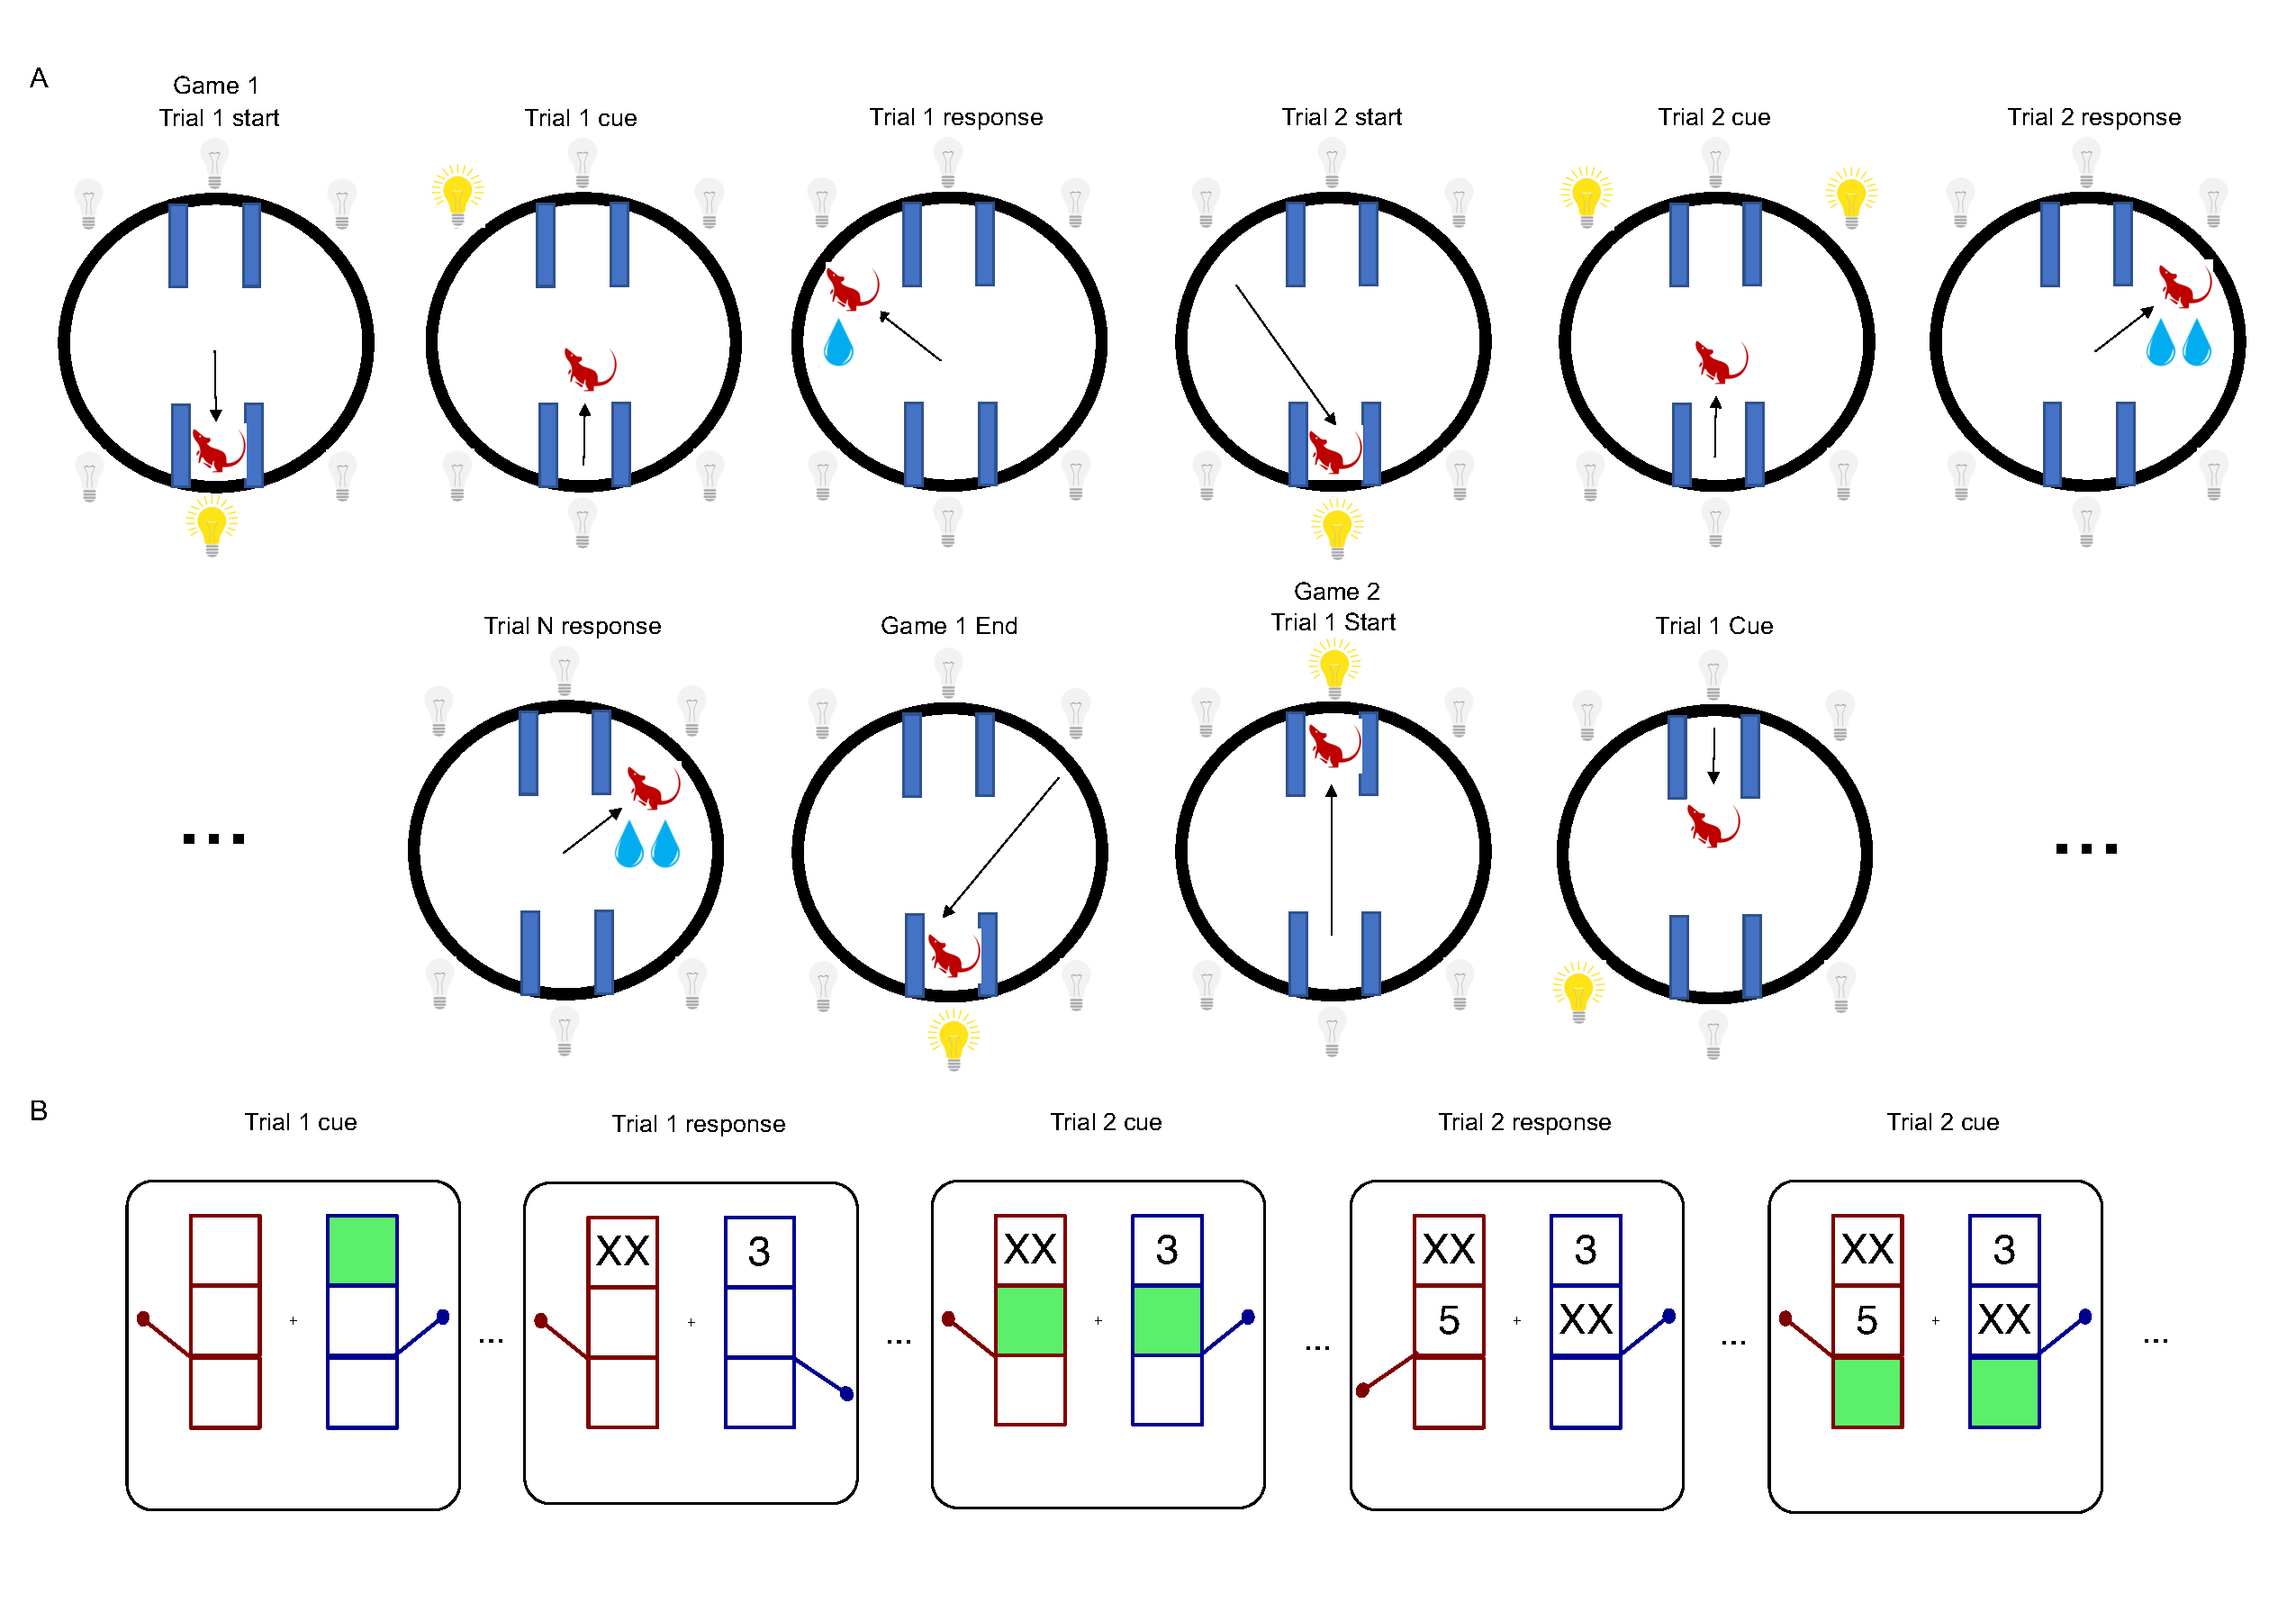
\includegraphics[width=1\textwidth]{figs/taskfigure.pdf}
			\caption{A. Rat version of the exploration task. B. Human version of the exploration task. }
			\label{fig:task}
	\end{center}
\end{figure}
\subsubsection*{Rat version}
% Rats are pre-trained that light is associated with reward. 
In this task, rats chose between two feeder locations that give out different amount of sugar water released in drops. The two feeders are associated with a fixed number of sugar water drawn uniformly from 0 to 5 in each game, and will always give the same number of drops of sugar water during a game whereas the reward magnitude (number of drops) will be reset before the start of a new game. In each game, before making their free choices, they were guided to one of the target feeders first in the first trial. From the 2nd trial, they are cued to make free choices for either 1 trial (short horizon condition) or 6 trials (long horizon condition). 

There are 4 feeder locations and 2 home bases in the experiment setup (See Figure \ref{fig:task}, A). The home base is placed between 2 lego blocks to separate them from the target feeders. Each home base is paired with the 2 feeders at the opposite side of the table. Each game will be played with one of the home bases and its associated target feeders. The other set of home base and feeders will be used for the next game. An LED light is set up at all 6 locations to cue the rats, and rats are pre-trained to follow lights. During the first trial of each game, the LED light will blink at one of the home bases, once the rat goes to the home base, the light will turn off and LED light at one of the target feeders will blink, and the rat is guided to visit that feeder, after which the cue light will come off and a certain number of sugar water drops will be released. From the second trial, after the rat is cued to go back to the home base, LED lights at both target feeders will blink simultaneously and the rat is free to go to either one. As soon as the rat makes its decision, both lights will come off and the rat will get the associated reward at the feeder visited. After the last choice is made, the rat is guided back to the home base and an 8s increasing tone is played to indicate the start of a new game,  after 10s (2s without sound) the light at the opposite will blink, and the next game begins.

Each home base is associated with a fixed horizon on each single session, and the association horizon condition will be reset pseudorandomly from session to session. % A decreasing tone is played every time the rat visits the home base to cue the rat about the horizon...

\subsubsection*{Human version}
In this task, participants are asked to choose between two slots machines (will also refer to as bandits) that give out a fixed number of rewards uniformly drawn from 1 to 5.  Participants are instructed to maximize the total points they get. The height of the boxes indicate the number of choices to make ( i.e. the horizon condition) in a game (See Figure \ref{fig:task} B), each row represents a trial. Before participants make their own choices, in the very first trial, they are asked to pick one of the bandits. The options available is highlighted with a green background color. For the first trial, only one of the two options will be highlighted and be available to choose. Participants indicate their choices by pressing the arrow keys on a keyboard. From the 2nd trial, both of the options will be available and participants are free to make their own choices. There are four horizon conditions (1, 2, 5, 9 free choices) and games with different horizons are interleaved. 


%\subsection*{Descriptive Model}
%	$$\Delta Q = \Delta R^t + \beta_{information} * \Delta I + \beta_{side} + \beta_{homebase} + \beta_{habit}  * side_{previous}$$
%	
%	where $$ \Delta R = R^t_{right} - R^t_{left}$$
%	$$R^t = R^{t-1} + \alpha (r^t - R^t) $$


\section*{Results}
\subsection*{Performance on the task}
\begin{figure}[H]
	\begin{center}
			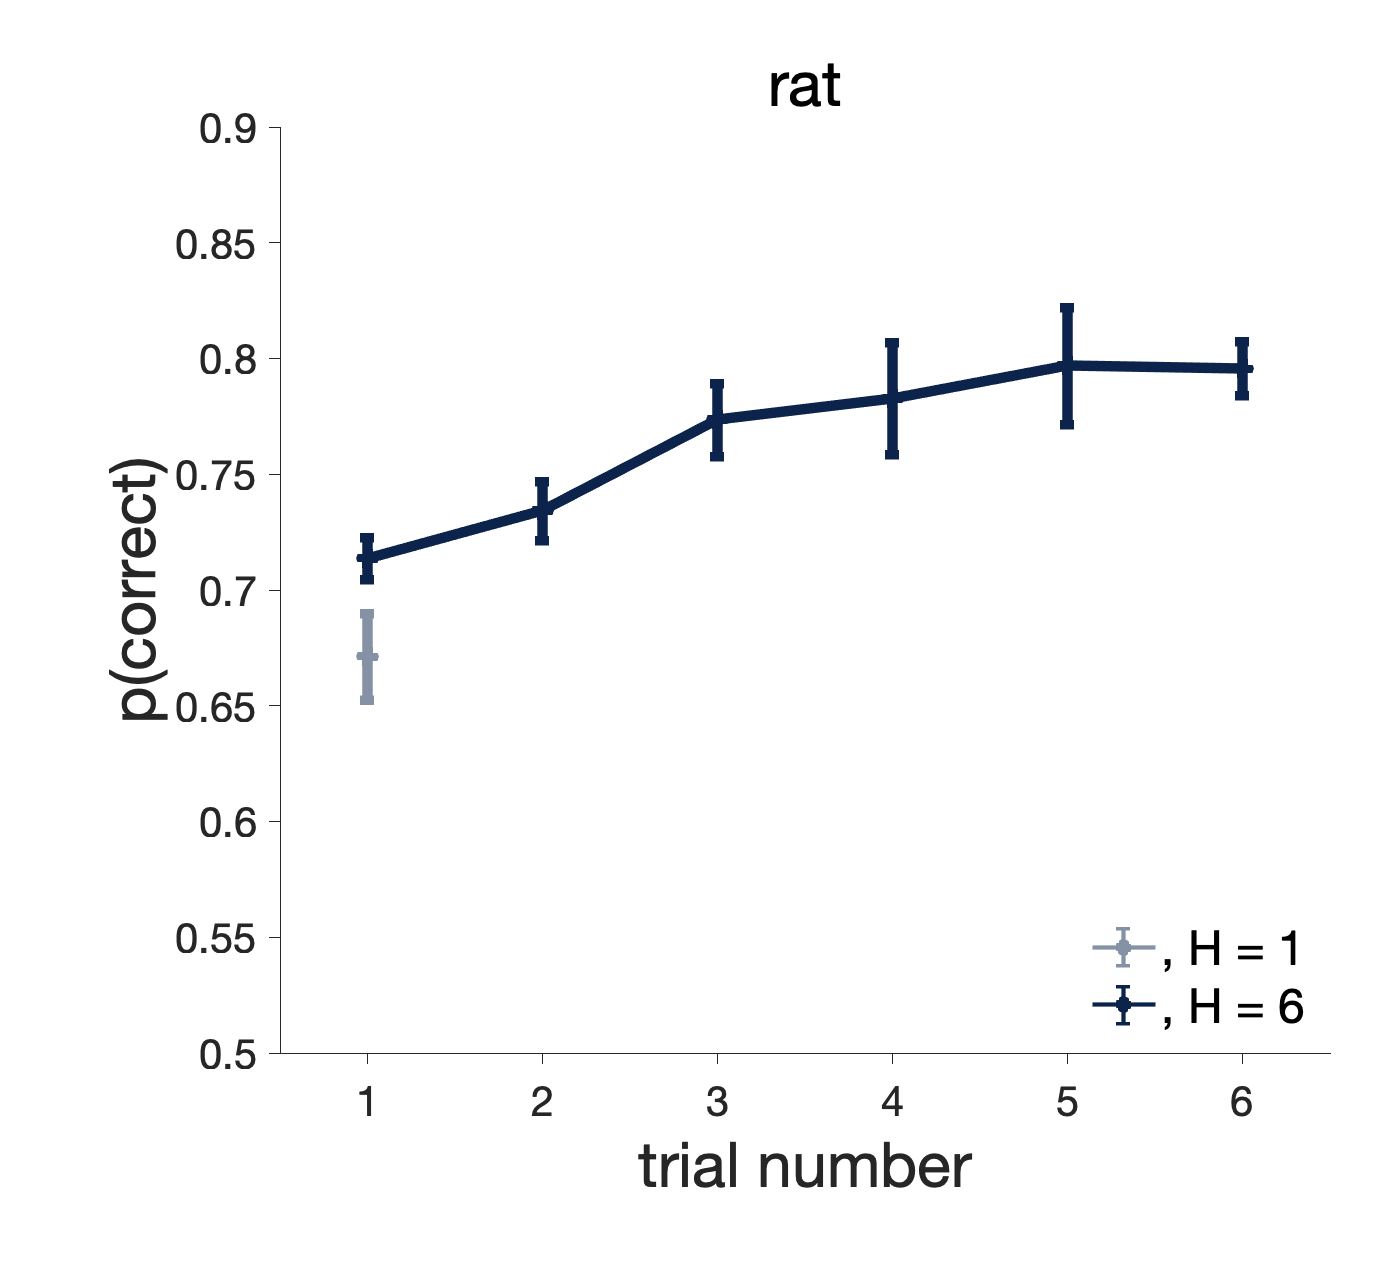
\includegraphics[width=0.4\textwidth]{figs/RatEE_performance.png}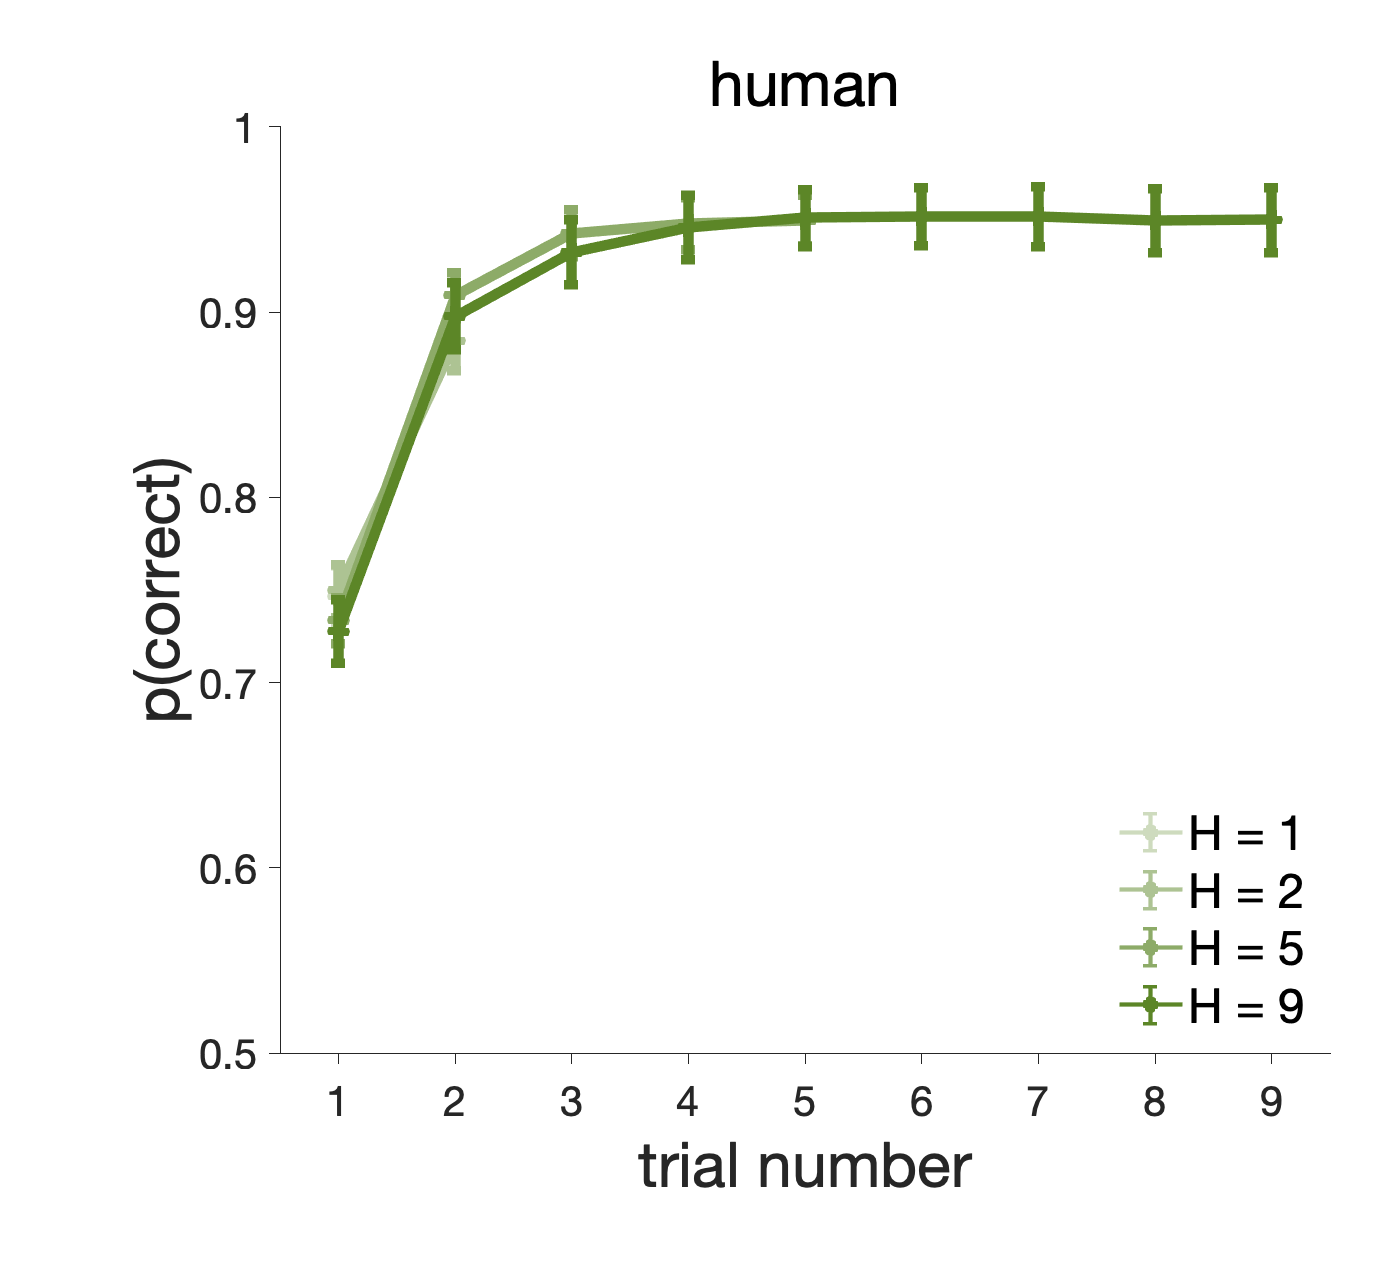
\includegraphics[width=0.4\textwidth]{figs/OneshotHuman_performance.png}
			\caption{Performance of rats and humans in the exploration task.}
	\end{center}
\end{figure}
\subsection*{Exploration as a function of exploit value}
\begin{figure}[H]
	\begin{center}
			\includegraphics[width=0.4\textwidth]{figs/RatEE_Free_pexplore.png}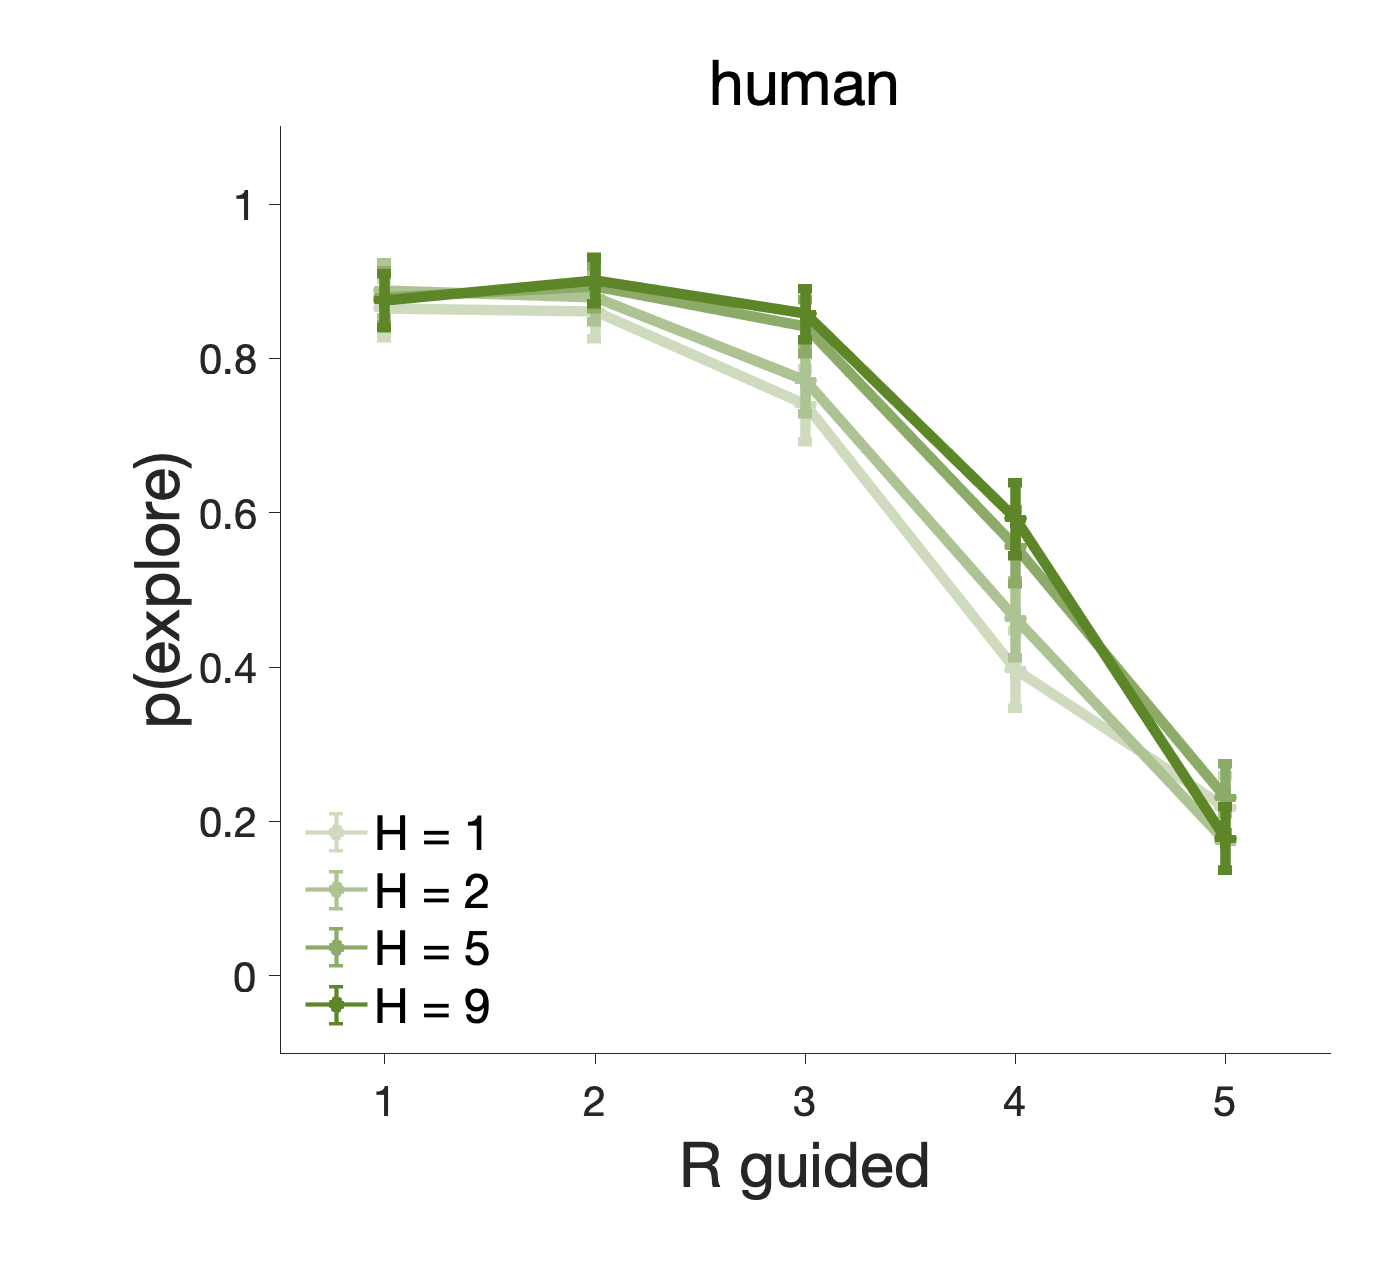
\includegraphics[width=0.4\textwidth]{figs/OneshotHuman_pexplore.png}
			\caption{P(explore).}
	\end{center}
\end{figure}

This task is very easy for humans, they can achieve an accuracy of 95\%, rats can learn  it as well with an accuracy of 80\%. Humans achieve a 90\% accuracy from the 2nd trial whereas rats learn gradually as they go in the task.\\

Both rats and humans chose to explore more when the exploit value is low. This is an indication of using the win-stay-lose-shift strategy. Humans increase the degree of exploration as horizon increases. However, the level of exploration doesn't seem to be modulated by horizon in rats. 



%\subsection*{Exploration as a function of horizon}
%\newpage
%\begin{figure}[H]
%	\begin{center}
%			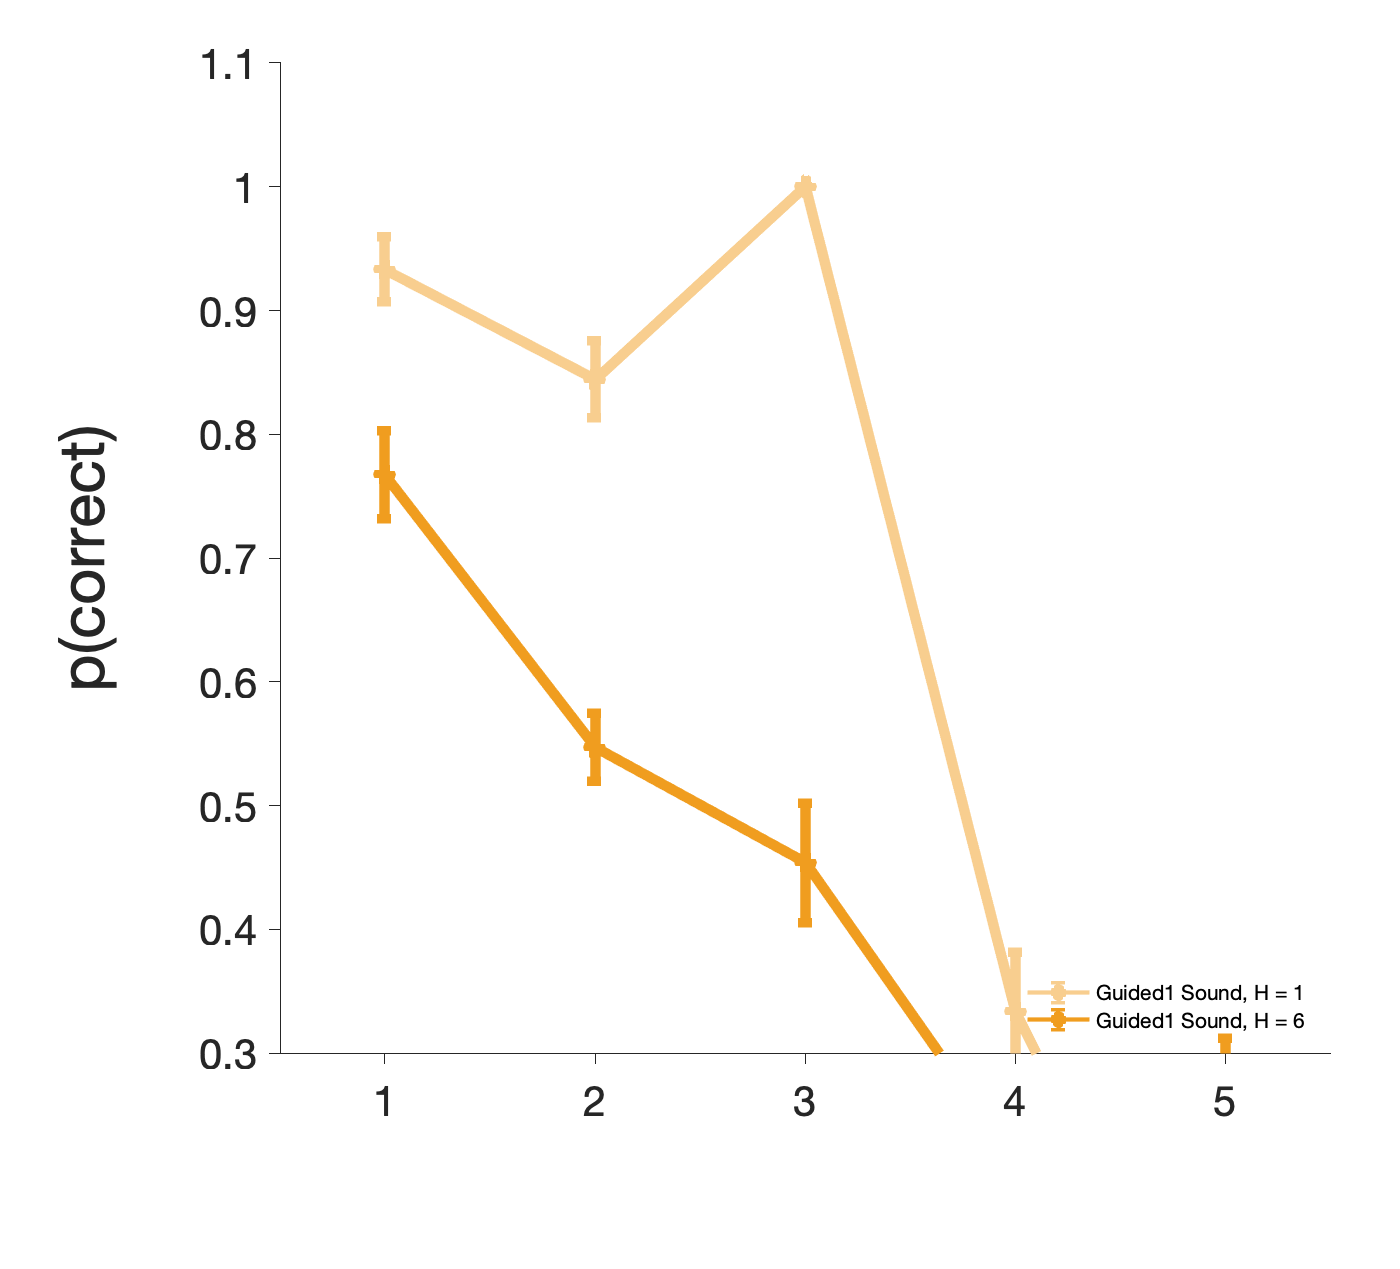
\includegraphics[width=1\textwidth]{figs/RatEE_ac2.png}
%			\caption{Accuracy by horizon.}
%	\end{center}
%\end{figure}%\begin{figure}[H]
%	\begin{center}
%			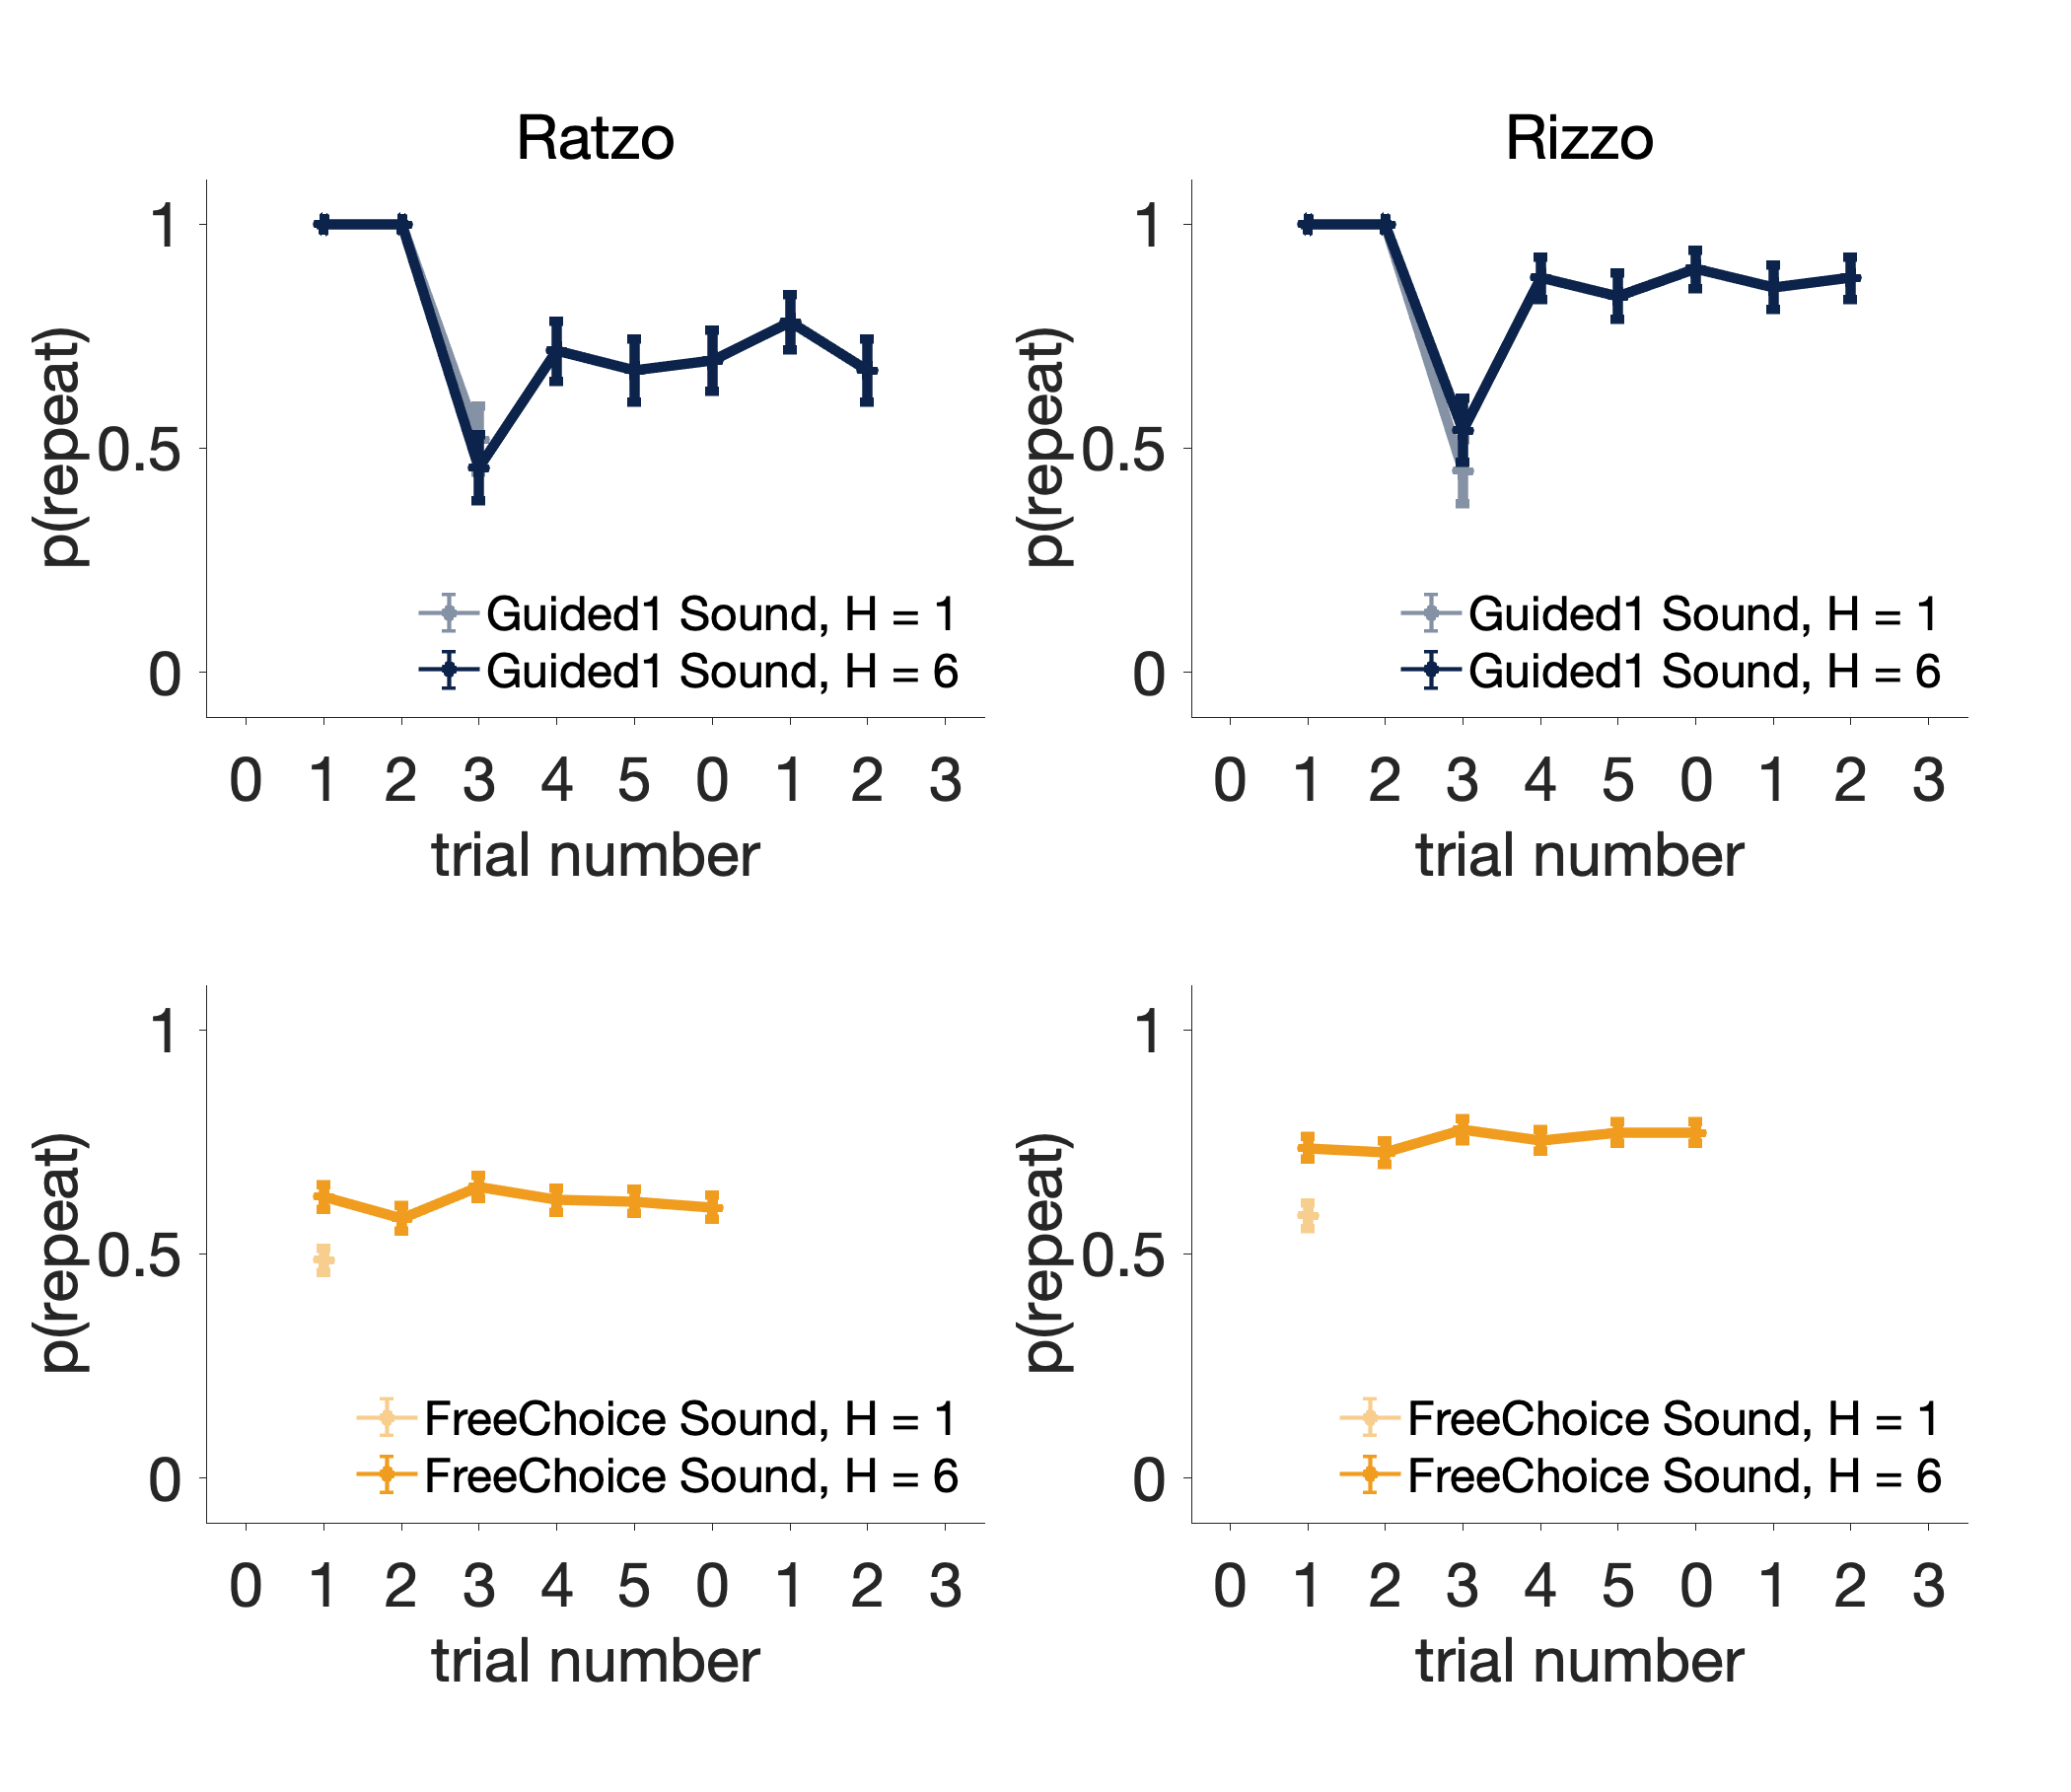
\includegraphics[width=1\textwidth]{figs/RatEE_pexplore_bytrial.png}
%			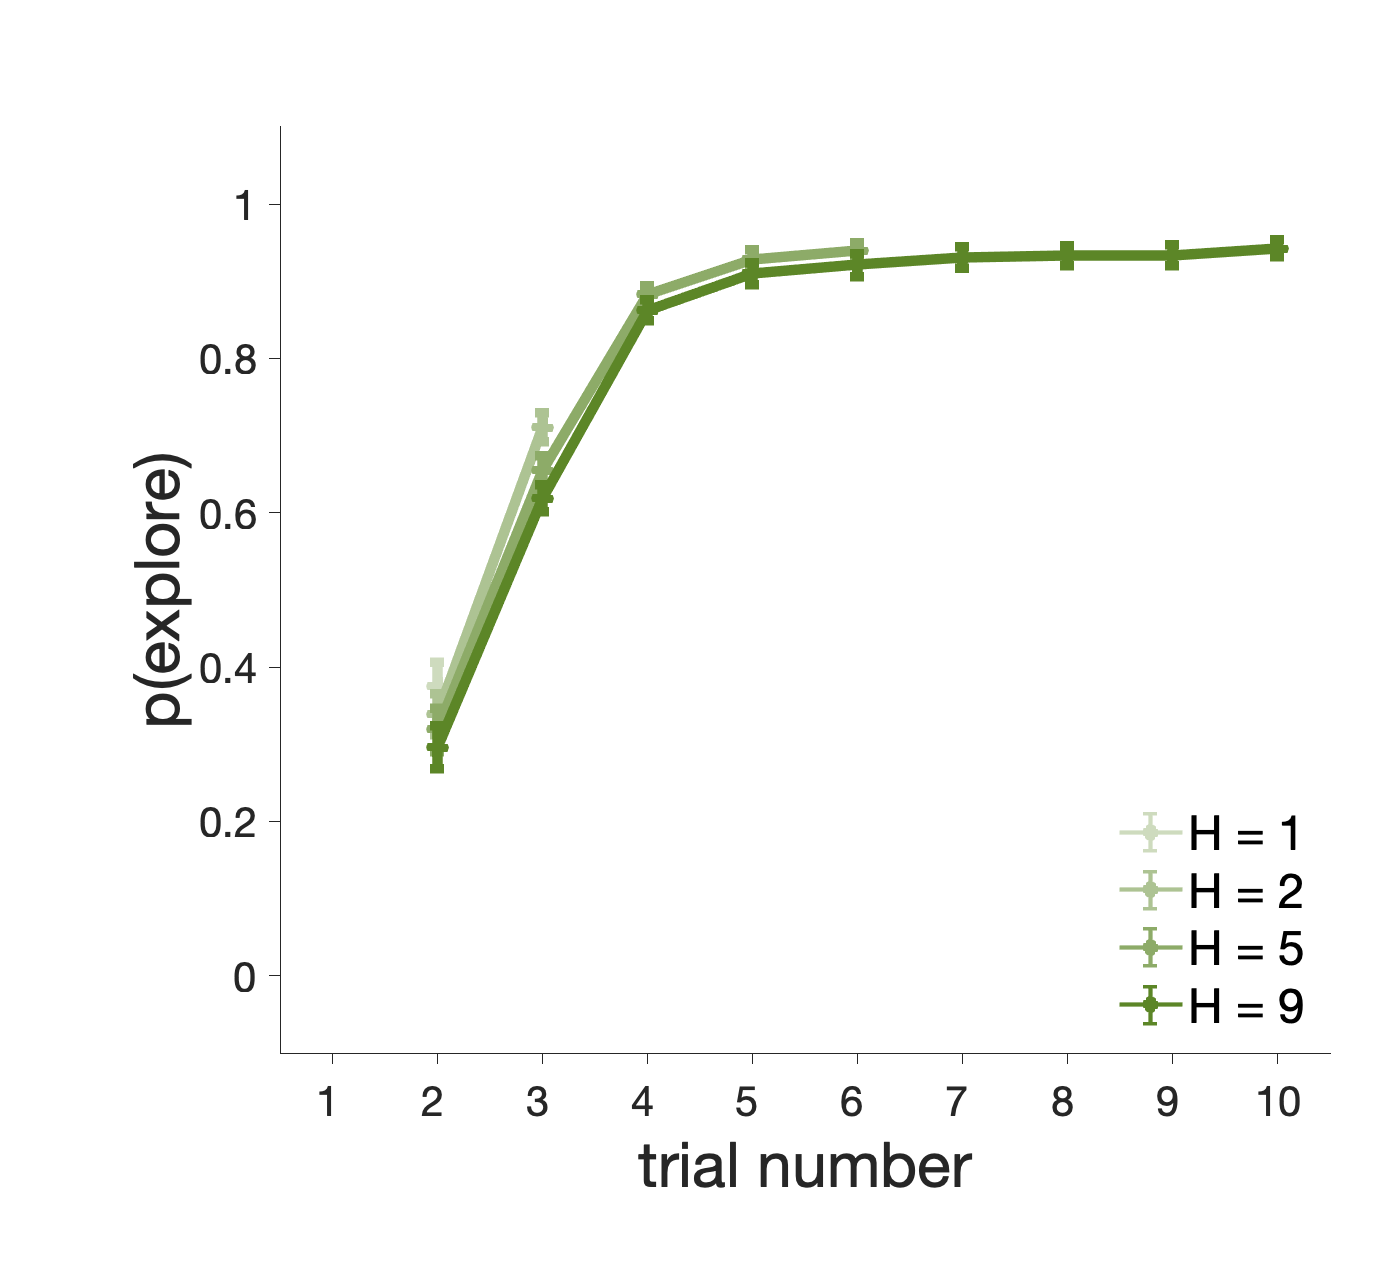
\includegraphics[width=0.5\textwidth]{figs/OneshotHuman_pexplore_bytrial.png}
%			\caption{P(explore).}
%	\end{center}
%\end{figure}

\section*{Discussion}

In this study, we designed a novelty seeking task to study explore-exploit decisions in rats. In this task, rats choose between a known option with fixed amount of reward, and an unknown option with an unknown fixed amount of reward. The extent to which they explore the unknown location in their initial choice serves as a measure of exploration. In particular, rats performed the task in both a short and a long horizon condition. Using an open-field, we are able to use two sets of different locations alternatively as new games start as opposed to having to reverse the reward conditions at the same set of locations. Using rewards of different magnitudes instead of probability, we are taking the uncertainty in the value estimate of actions out of the equation, and as a result, exploration can be defined in a clean way that dose not depend on modeling. By looking at the extent to which rats go to the unvisited location at their initial choices, we are able to directly quantify information-driven exploration. We also ran a human version of an identical task except that humans are choosing between two slot machines that give out different amount of reward points, so we are able to compare rodent behavior directly with humans in this task. Humans explore more in longer horizon context, whereas rats don't adapt the level of exploration to the horizon condition. 
\bibliographystyle{plainnat}
\bibliography{RatExploration_refs.bib}
\end{document}